\documentclass[journal]{IEEEtran}
\usepackage[a5paper, margin=10mm, onecolumn]{geometry}
\usepackage{lmodern} % Ensure lmodern is loaded for pdflatex
\usepackage{tfrupee} % Include tfrupee package

\setlength{\headheight}{1cm} % Set the height of the header box
\setlength{\headsep}{0mm}     % Set the distance between the header box and the top of the text

\usepackage{gvv-book}
\usepackage{gvv}
\usepackage{cite}
\usepackage{amsmath,amssymb,amsfonts,amsthm}
\usepackage{algorithmic}
\usepackage{graphicx}
\usepackage{textcomp}
\usepackage{xcolor}
\usepackage{txfonts}
\usepackage{listings}
\usepackage{enumitem}
\usepackage{mathtools}
\usepackage{gensymb}
\usepackage{comment}
\usepackage[breaklinks=true]{hyperref}
\usepackage{tkz-euclide} 
\usepackage{listings}                                      
\def\inputGnumericTable{}                                 
\usepackage[latin1]{inputenc}                                
\usepackage{color}                                            
\usepackage{array}                                            
\usepackage{longtable}
\usepackage{multicol}
\usepackage{calc}                                             
\usepackage{multirow}                                         
\usepackage{hhline}                                           
\usepackage{ifthen}                                           
\usepackage{lscape}
\begin{document}
	
	\bibliographystyle{IEEEtran}
	\vspace{3cm}
	
	\title{10.3.4.1.4}
	\author{EE24BTECH11008 - Aslin Garvasis}
	% \maketitle
	% \newpage
	% \bigskip
	{\let\newpage\relax\maketitle}
	
	\renewcommand{\thefigure}{\theenumi}
	\renewcommand{\thetable}{\theenumi}
	\setlength{\intextsep}{10pt} % Space between text and floats
	
	
	\numberwithin{equation}{enumi}
	\numberwithin{figure}{enumi}
	\renewcommand{\thetable}{\theenumi}
	
	
	\textbf{Question}:\newline
	Solve the following pair of of linear equation by the elimination method and substitution method:
    \begin{align}
        \frac{x}{2}+\frac{2y}{3}&=-1\\
        x-\frac{y}{3}&=3
    \end{align}
	\textbf{ Represent the system in matrix form} \\ 
The system of equations can be written as:  
\begin{align}  
A \mathbf{x} = \mathbf{b},  
\end{align}  
where  
\begin{align}  
A = \begin{pmatrix} \frac{1}{2} & \frac{2}{3} \\ 1 & \frac{-1}{3} \end{pmatrix}, \mathbf{x} = \begin{pmatrix} x \\ y \end{pmatrix}, \mathbf{b} = \begin{pmatrix} -1 \\ 3 \end{pmatrix}.  
\end{align}

\textbf{Perform LU Decomposition using Doolittle's Algorithm} \\ 
We decompose the matrix $A$ into the product of a lower triangular matrix $L$ and an upper triangular matrix $U$, i.e.,  
\begin{align}  
A = LU,  
\end{align}  
where  
\begin{align}
	L = \myvec{1 & 0 & 0 & \cdots & 0 \\ l_{21} & 1 & 0 & \cdots & 0 \\ l_{31} & l_{32} & 1 & \cdots & 0 \\ \vdots & \vdots & \vdots & \ddots & 0 \\ l_{n1} & l_{n2} & l_{n3} & \cdots & 1},\quad
	U = \myvec{u_{11} & u_{12} & u_{13} & \cdots & u_{1n} \\ 0 & u_{22} & u_{23} & \cdots & u_{2n} \\ 0 & 0 & u_{33} & \cdots & u_{3n} \\ \vdots & \vdots & \vdots & \ddots & u_{n-1,n} \\ 0 & 0 & 0 & \cdots & u_{nn}}.
\end{align}
 The elements of these matrices are calculated as follows: \\  
Elements of the $U$ Matrix: \\  
For each column $j$:  
\begin{align}  
U_{ij} = A_{ij} \text{ if } i = 0, \\  
U_{ij} = A_{ij} - \sum_{k=0}^{i-1} L_{ik} U_{kj} \text{ if } i > 0.  
\end{align}  
Elements of the $L$ Matrix: \\  
For each row $i$:  
\begin{align}  
L_{ij} = \frac{A_{ij}}{U_{jj}} \text{ if } j = 0, \\  
L_{ij} = \frac{A_{ij} - \sum_{k=0}^{j-1} L_{ik} U_{kj}}{U_{jj}} \text{ if } j > 0.  
\end{align}  

\begin{align}  
L = \begin{pmatrix} 1 & 0 \\ l_{21} & 1 \end{pmatrix}, U = \begin{pmatrix} u_{11} & u_{12} \\ 0 & u_{22} \end{pmatrix}.  
\end{align}

Now, let's compute the LU decomposition step by step.  

First, we find the elements of $U$ and $L$:  
\begin{align}  
u_{11} = a_{11} = \frac{1}{2}, u_{12} = a_{12} = \frac{2}{3}.  
\end{align}  
Next, we compute $l_{21}$ and $u_{22}$:  
\begin{align}  
l_{21} = \frac{a_{21}}{u_{11}} = \frac{1}{\frac{1}{2}} = 2,  
\end{align}  
\begin{align}  
u_{22} = a_{22} - l_{21} u_{12} = \frac{-1}{3} - 2 \times (\frac{2}{3}) = \frac{-5}{3}.  
\end{align}  
So the LU decomposition is:  
\begin{align}  
L = \begin{pmatrix} 1 & 0 \\ 2 & 1 \end{pmatrix}, U = \begin{pmatrix} \frac{1}{2} & \frac{2}{3} \\ 0 & \frac{-5}{3} \end{pmatrix}.  
\end{align}

\textbf{Solve for $\mathbf{x}$ using $LU$ decomposition}  \\
Now we solve the system in two steps using forward substitution and backward substitution.  

First, solve $L \mathbf{y} = \mathbf{b}$ for $\mathbf{y}$:  
\begin{align}  
\begin{pmatrix} 1 & 0 \\ 2 & 1 \end{pmatrix} \begin{pmatrix} y_1 \\ y_2 \end{pmatrix} = \begin{pmatrix} -1 \\ 3 \end{pmatrix}.  
\end{align}  
This gives:  
\begin{align}  
y_1 = -1
\end{align}
\begin{align}
2y_1 + y_2 = 3 \Rightarrow 2(-1) + y_2 = 3 \Rightarrow y_2 = 5.  
\end{align}  
Thus, $\mathbf{y} = \begin{pmatrix} -1 \\ 5 \end{pmatrix}$.  

Next, solve $U \mathbf{x} = \mathbf{y}$ for $\mathbf{x}$:  
\begin{align}  
\begin{pmatrix} \frac{1}{2} & \frac{2}{3} \\ 0 & \frac{-5}{3} \end{pmatrix} \begin{pmatrix} x \\ y \end{pmatrix} = \begin{pmatrix} -1 \\ 5 \end{pmatrix}.  
\end{align}  
This gives:  
\begin{align}  
\frac{-5}{3}y = 5 \Rightarrow y = -3,  
\end{align}  
\begin{align}  
\frac{1}{2}x + \frac{2}{3}y = -1 \Rightarrow \frac{1}{2}x + \frac{2}{3}\times -3 = -1 \Rightarrow x = 2.  
\end{align}  

Thus, the solution is $x = 2$ and $y = -3$.  

 
\begin{figure}[h!]
   \centering
   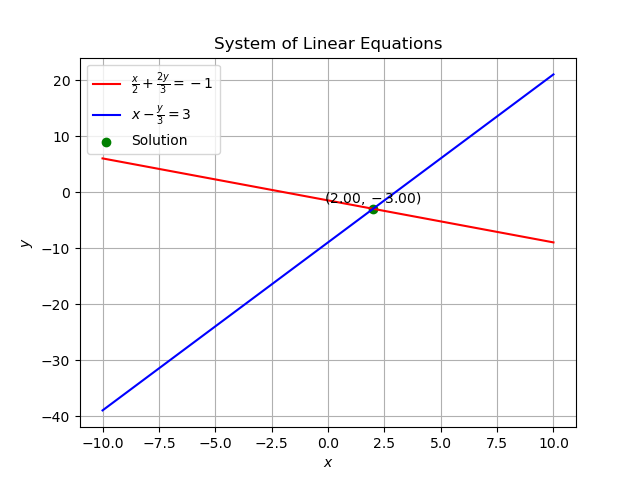
\includegraphics[width=1\columnwidth]{figs/Fig1.png}
   \caption{Solving the system of equations}
   \label{stemplot}
\end{figure}


\end{document}


\end{document}
